% --------------------------------------------------- 
% Scat Model
% --------------------------------------------------- 
\section{Scat Model}
\subsection{}

\begin{frame}
\frametitle{Model Basics}

We assume a multinomial error structure

\begin{align*}
p(y_{l \cdot k}|f_{l \cdot k}) = \frac{s_{lk}!}{\prod_i y_{lik}!} \prod_i (f_{lik})^{y_{lik}}
\end{align*}

where:\\

\begin{itemize}
\item $f_{lik}$ is the allele frequency of allele $i$ from locus $l$ at location $k$.
\item $y_{lik}$ is the count of allele $i$ from locus $l$ at location $k$.
\item $s_{lk} = \sum_i y_{lik}$ is the total count of alleles from locus $l$ at location $k$.
\end{itemize}

\end{frame}


\begin{frame}
\frametitle{Modeling allele frequency}


We model allele frequency using values from a normalized, $\sum_i f_{lik} = 1$, Gaussian Process:\\
\[
f_{lik} = \frac{\exp(\theta_{lik})}{\sum_j \exp(\theta_{ljk})}
\]

where
\[
\underset{[r \times 1]}{\bm{\theta}_{li}} \sim \text{MVN}( \underset{[r \times 1]}{\bm{M}_{li}}, \underset{[r \times r]}{\bm{\Sigma_{}}})
\]

\end{frame}

\begin{frame}
\frametitle{Mean of $\bm\theta$}

\begin{align*}
\underset{[r \times 1]}{\bm{M}_{li}} &=  \xi_l ~ \eta_{li} ~ \bm{1}_{[r,1]}\\\\
\xi_l &\sim \text{Unif}(-\infty,\infty)\\\\
\eta_{li} &\sim \text{N}(0,\beta_l)\\
\beta_l &\sim \text{Unif}(0,10^6)\\
\end{align*}

{\footnotesize
*Overparameterization using $\xi$ is included in the model as it increases the speed of convergence
}
\end{frame}


\begin{frame}
\frametitle{Variance of $\bm\theta$}

We assume that the process is stationary and isotropic, therefore $\bm\Sigma$ only depends on the distance between locations.

\begin{align*}
\{\bm\Sigma\}_{k_1,k_2} &= \sigma(d_{k_1,k_2})
\end{align*}

where $\sigma(d)$ is defined by a covariance function.

\vspace{2mm}



\end{frame}



\begin{frame}
\frametitle{Covariance Functions}

Powered Exponential Covariance:
\[
\sigma(d|\bm\alpha) = \alpha_0 \exp\left[-\left(\frac{d}{\alpha_1}\right)^{\alpha_2}\right] + \alpha_3 \; I_{d=0}
\] 

Mat\'ern Covariance:
\[
\sigma(d|\bm\alpha) = \alpha_0 \frac{1}{\Gamma(\alpha_2)\;2^{(\alpha_2-1)}} \left(\frac{d}{\alpha_1}\right)^{\alpha_2} K_{\alpha_2}\left(\frac{d}{\alpha_1}\right)+ \alpha_3 \; I_{d=0}
\]

with the following priors on $\bm \alpha$:
\[ \alpha_0, \log(\alpha_1), \log(\alpha_2), \alpha_3 \sim \text{Unif}\]
\end{frame}



\begin{frame}
\frametitle{Model Fitting via MCMC}

All parameters are updated by random walk Metropolis Hasting with normal jump proposals.\\
\vspace{5mm}
However, we first reparameterize as follows:
\begin{align*}
\underset{[r \times 1]}{\bm V_{li}} &\sim \text{MVN}(0,\underset{[r \times r]}{\bm\Sigma_{}}) \\
\underset{[r \times 1]}{\bm V_{li}} &= \underset{[r \times r]}{\text{Chol}(\bm\Sigma)} \cdot \underset{[r \times 1]}{\bm X_{li}}
\end{align*}

where

\[ \{\bm X_{li}\}_k \sim \text{N}(0,1) \]

\end{frame}



\begin{frame}
\frametitle{Alpha Traces}
\begin{center}
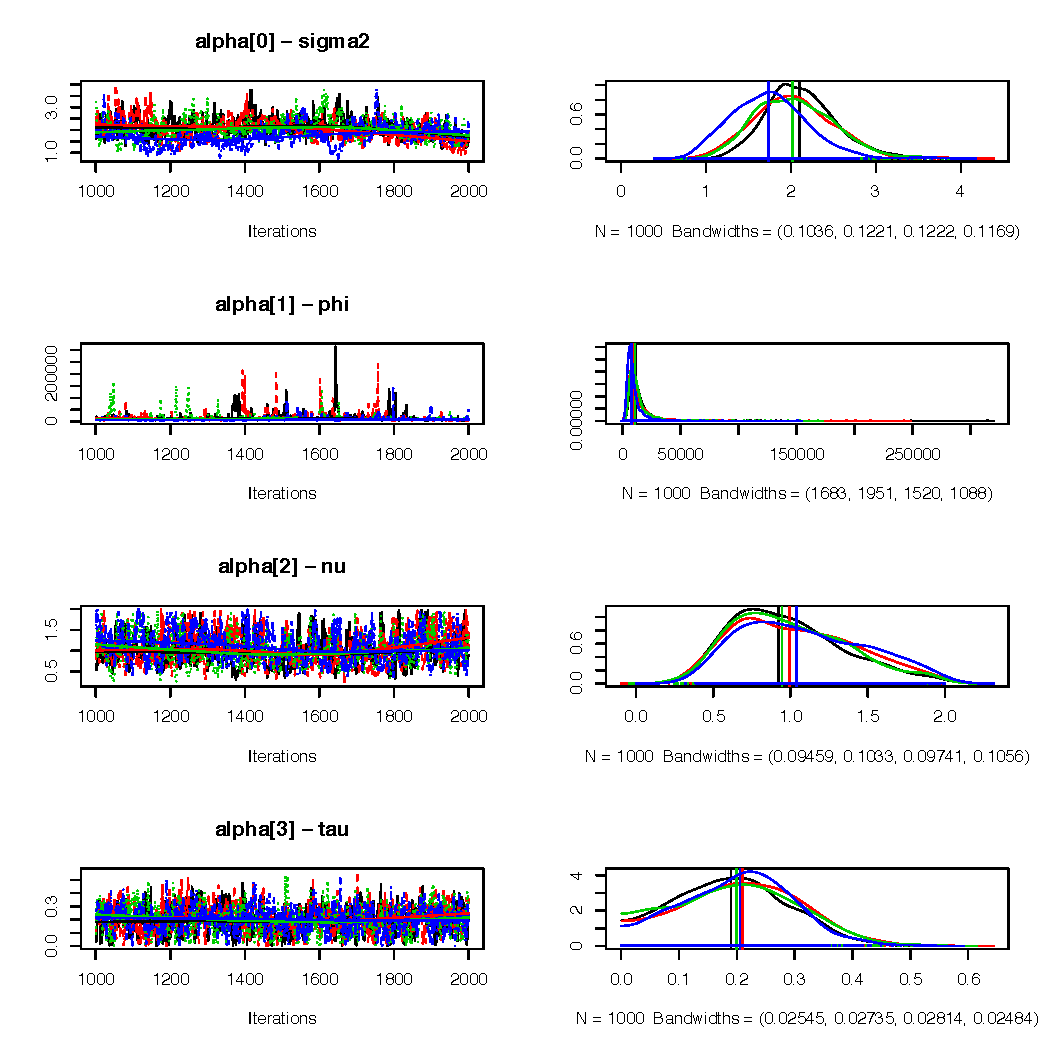
\includegraphics[width=2.5in]{scat/pics/mcmc-alpha.pdf}\\
\end{center}
\end{frame}



\begin{frame}
\frametitle{Allele Frequency - Hermit Thrush Locus 3 - Mean}

\begin{changemargin}{2cm}{-6.5cm}
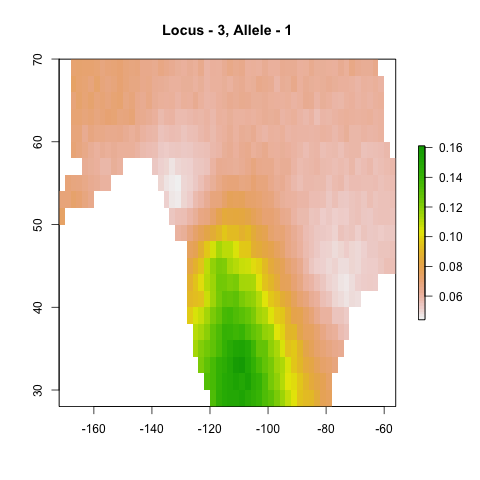
\includegraphics[width=0.9in]{scat/pics/Mean-Al3-1.png}
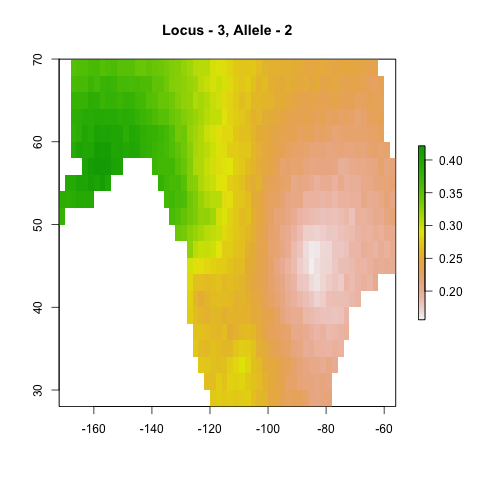
\includegraphics[width=0.9in]{scat/pics/Mean-Al3-2.png}
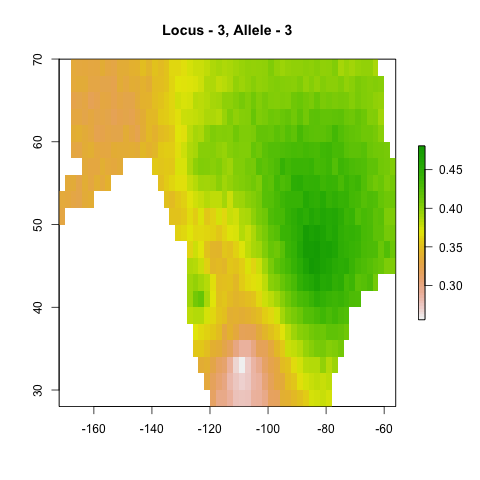
\includegraphics[width=0.9in]{scat/pics/Mean-Al3-3.png} \\
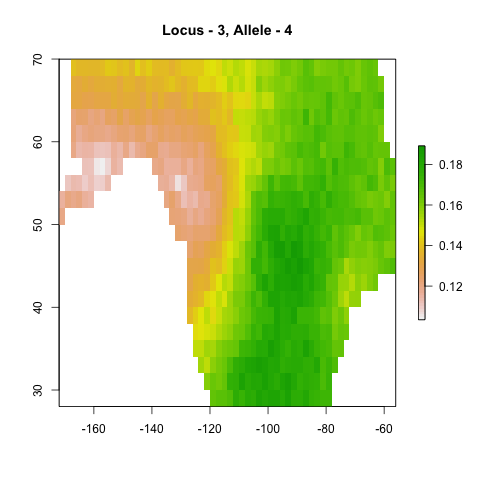
\includegraphics[width=0.9in]{scat/pics/Mean-Al3-4.png}
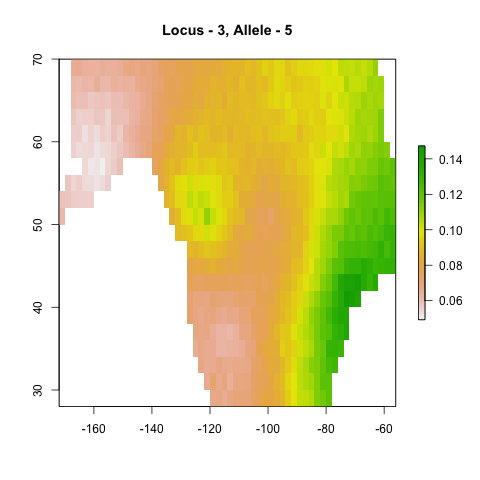
\includegraphics[width=0.9in]{scat/pics/Mean-Al3-5.png} 
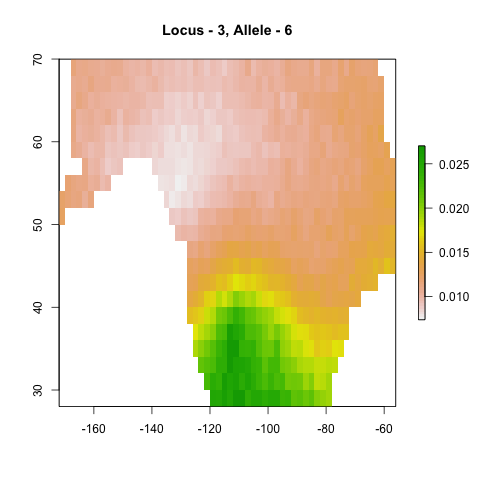
\includegraphics[width=0.9in]{scat/pics/Mean-Al3-6.png} \\
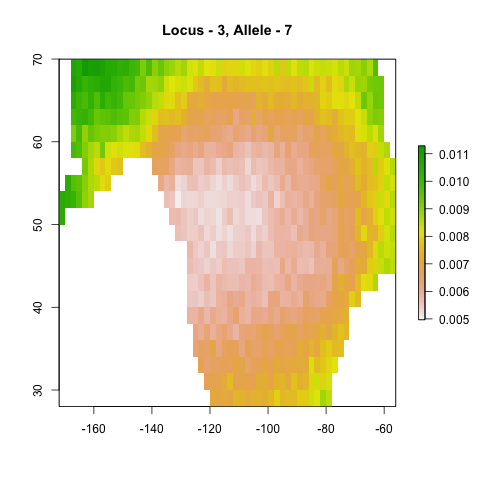
\includegraphics[width=0.9in]{scat/pics/Mean-Al3-7.png}
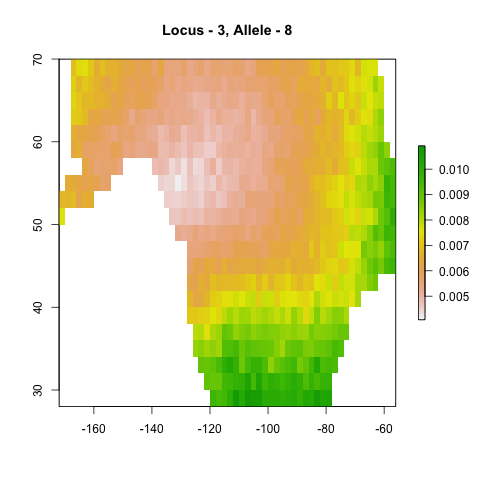
\includegraphics[width=0.9in]{scat/pics/Mean-Al3-8.png}
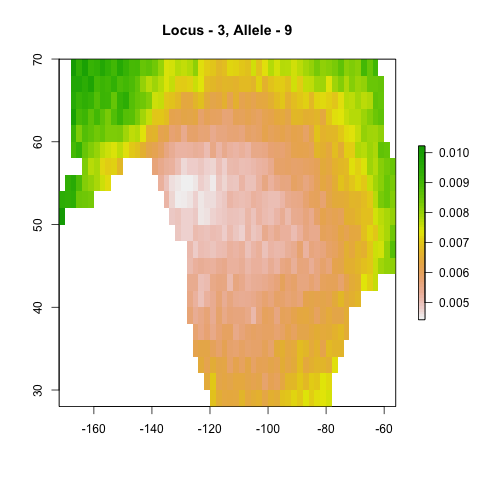
\includegraphics[width=0.9in]{scat/pics/Mean-Al3-9.png}
\end{changemargin}

\end{frame}


\begin{frame}
\frametitle{Allele Frequency - Hermit Thrush Locus 3 - Median}

\begin{changemargin}{2cm}{-6.5cm}
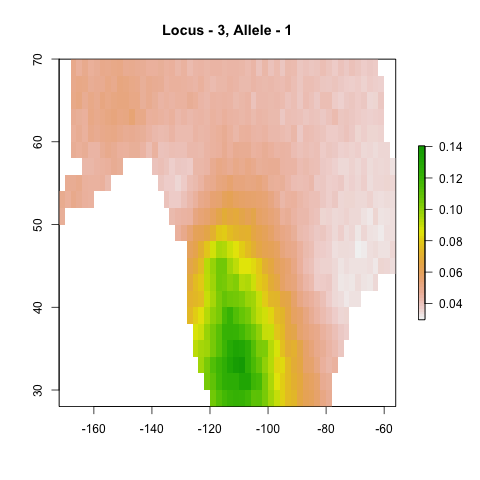
\includegraphics[width=0.9in]{scat/pics/Med-Al3-1.png}
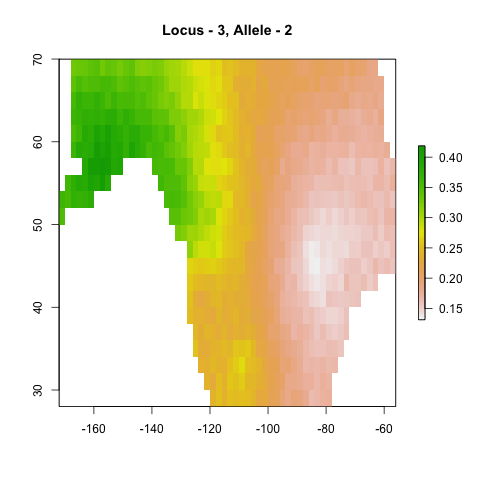
\includegraphics[width=0.9in]{scat/pics/Med-Al3-2.png}
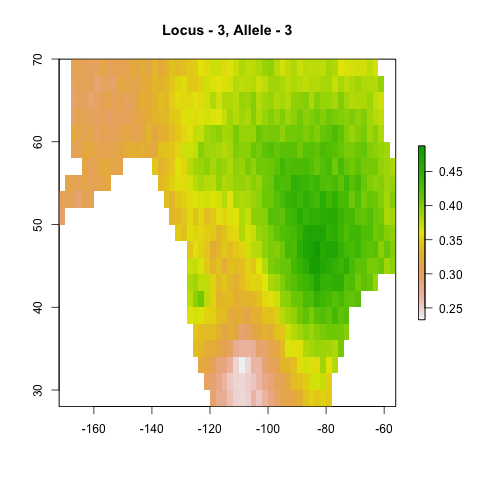
\includegraphics[width=0.9in]{scat/pics/Med-Al3-3.png} \\
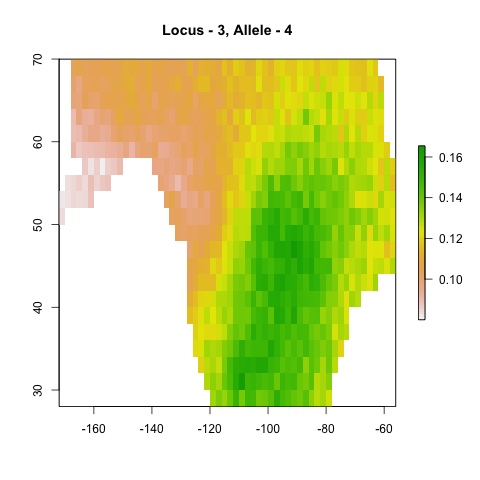
\includegraphics[width=0.9in]{scat/pics/Med-Al3-4.png}
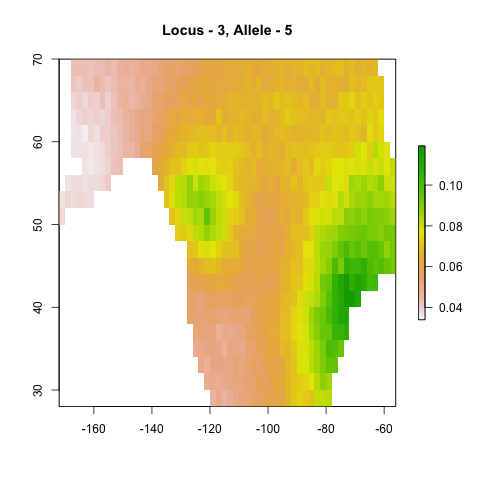
\includegraphics[width=0.9in]{scat/pics/Med-Al3-5.png} 
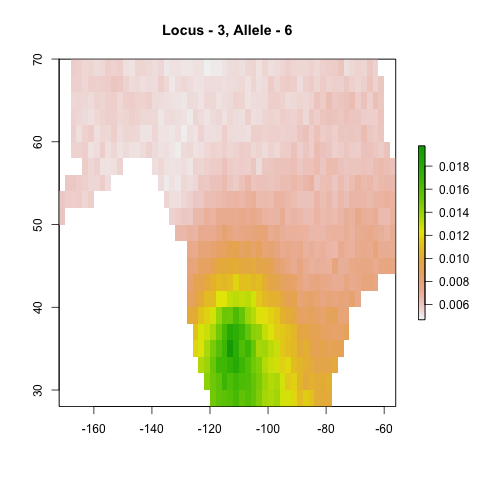
\includegraphics[width=0.9in]{scat/pics/Med-Al3-6.png} \\
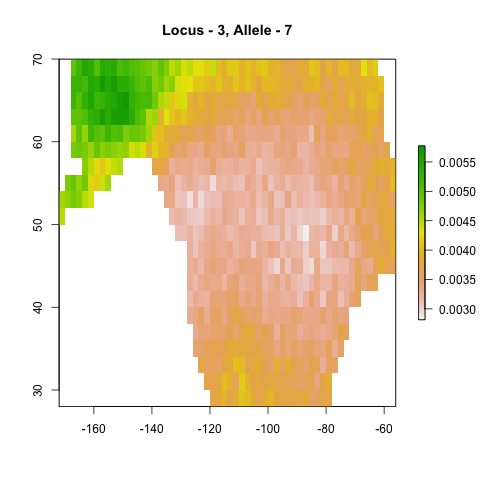
\includegraphics[width=0.9in]{scat/pics/Med-Al3-7.png}
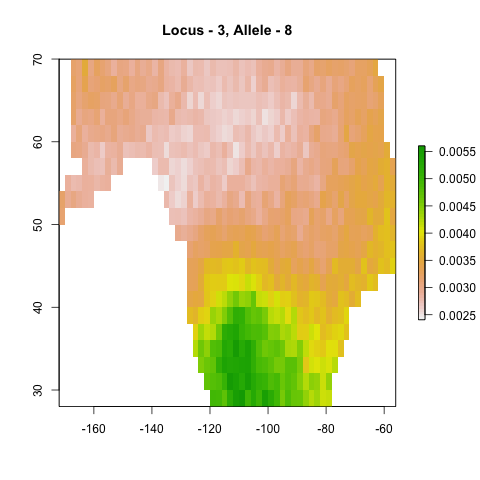
\includegraphics[width=0.9in]{scat/pics/Med-Al3-8.png}
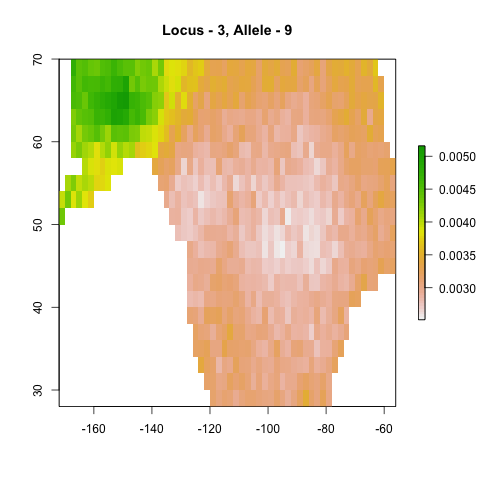
\includegraphics[width=0.9in]{scat/pics/Med-Al3-9.png}
\end{changemargin}

\end{frame}




\begin{frame}
\frametitle{Deviance Traces}

\vspace{-3mm}

%\begin{center}
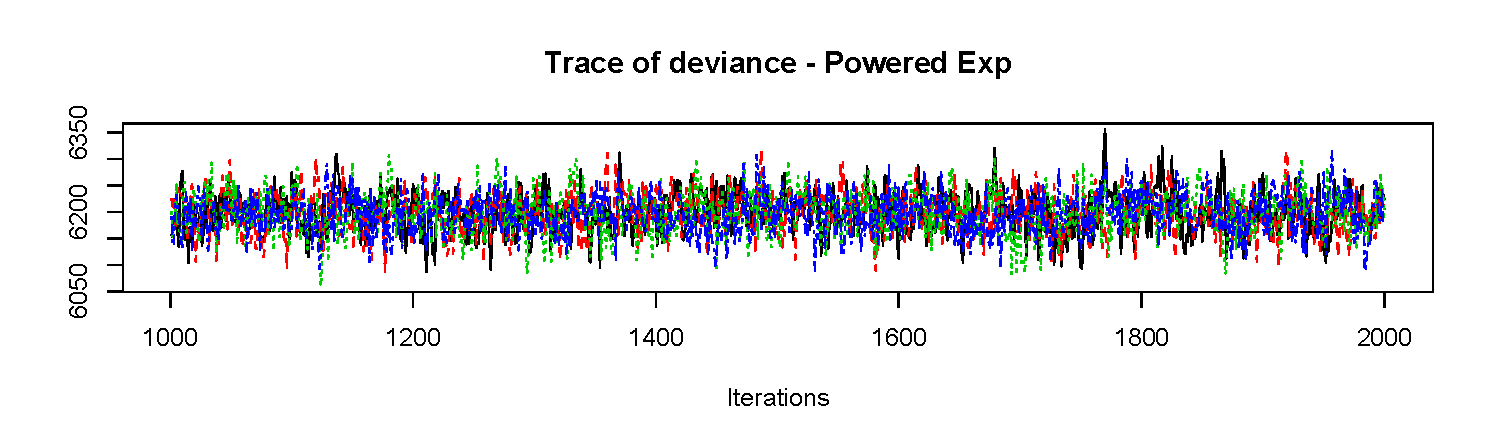
\includegraphics[width=4.5in]{scat/pics/deviance-poweredexp.pdf}\\
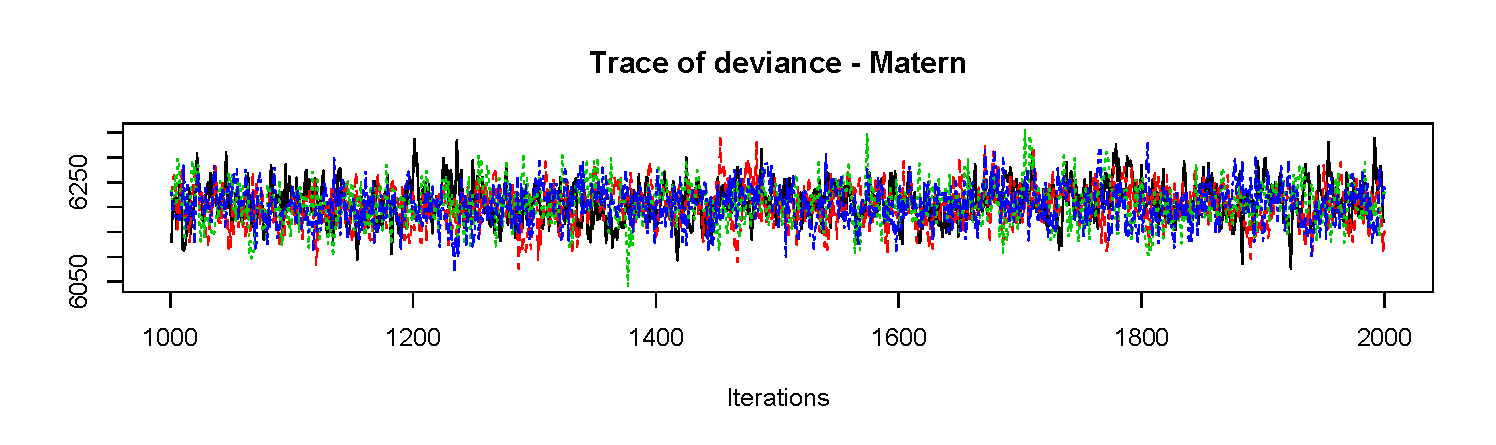
\includegraphics[width=4.5in]{scat/pics/deviance-matern.pdf}
%\end{center}
\end{frame}



\begin{frame}
\frametitle{Likelihood of an Individual}
For an individual $I$ from location $k$ with alleles $i_l$ and $j_l$ at locus $l$
\begin{align*}
p(I | f,k) &= \prod_l p_l(i_l,j_l|f,k)\\
p_l(i_l,j_l|f,k) &= \begin{cases} 
\gamma \; p_l(i_l|f,k) + (1-\gamma) \; p_l(i_l|f,k)^2   & \text{ if } i_l = j_l \\
(1-\gamma) \; p(i_l|f,k) \; p(j_l|f,k)                  & \text{ if } i_l \neq j_l \\
\end{cases} \\\\
p_l(i_l|f,k) &= (1-\delta) f_{lik} + \delta / m_l
\end{align*}

where $\delta$ is the probability only one of the alleles amplified and $\gamma$ is the probability of a genotyping error.

\end{frame}


% --------------------------------------------------- 
% HETH
% --------------------------------------------------- 

\section[Results]{Results - Hermit Thrush}
\subsection{}


\begin{frame}
\frametitle{Spatial Posterior - Individual 1}
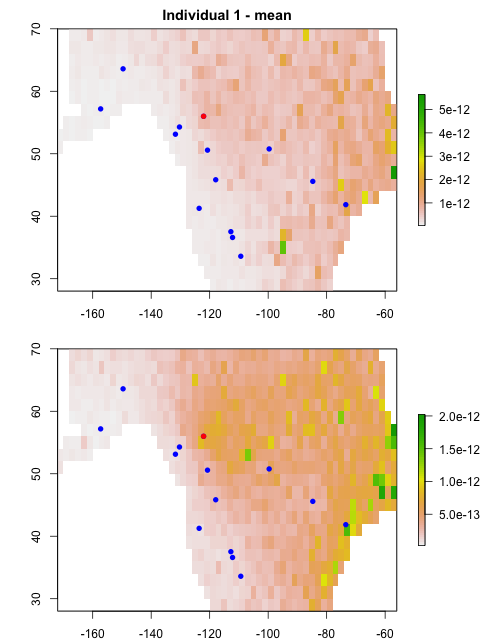
\includegraphics[width=2in]{scat/pics/Ind1-mean.png}
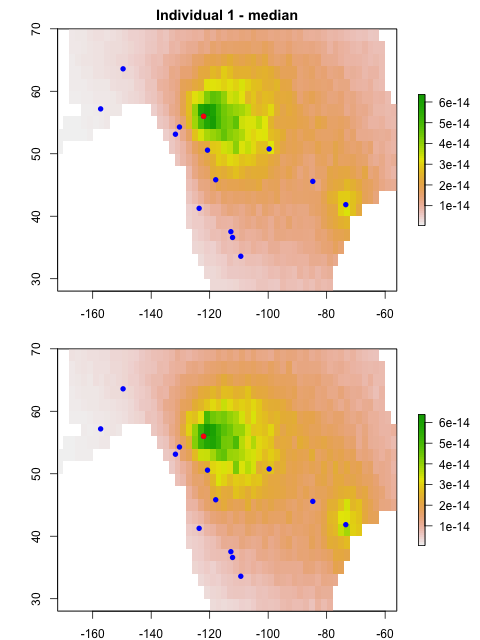
\includegraphics[width=2in]{scat/pics/Ind1-median.png}
\end{frame}

\begin{frame}
\frametitle{Spatial Posterior - Individual 37}
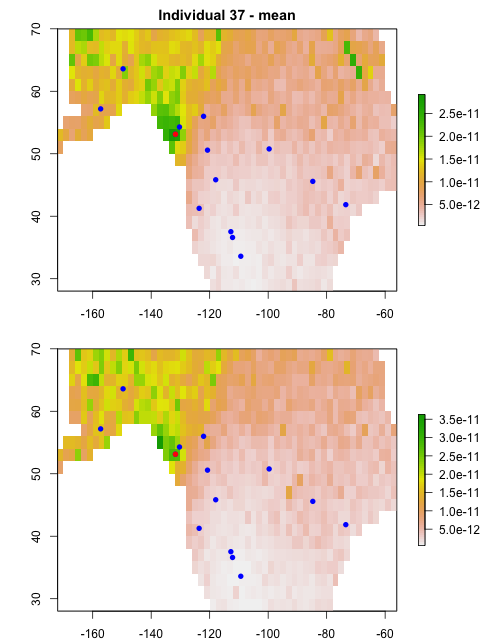
\includegraphics[width=2in]{scat/pics/Ind37-mean.png}
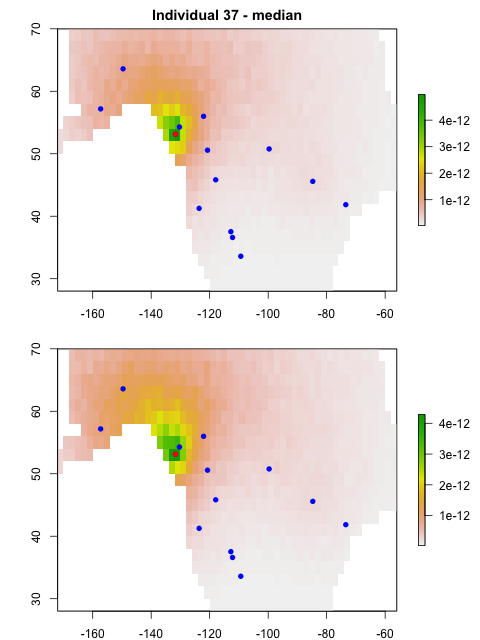
\includegraphics[width=2in]{scat/pics/Ind37-median.png}
\end{frame}

\begin{frame}
\frametitle{Spatial Posterior - Individual 93}
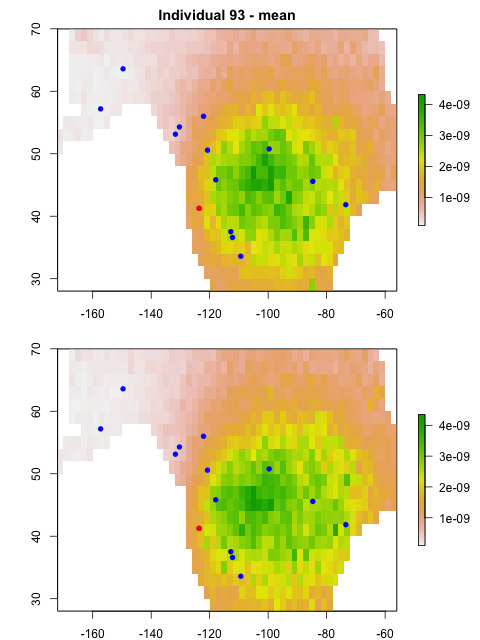
\includegraphics[width=2in]{scat/pics/Ind93-mean.png}
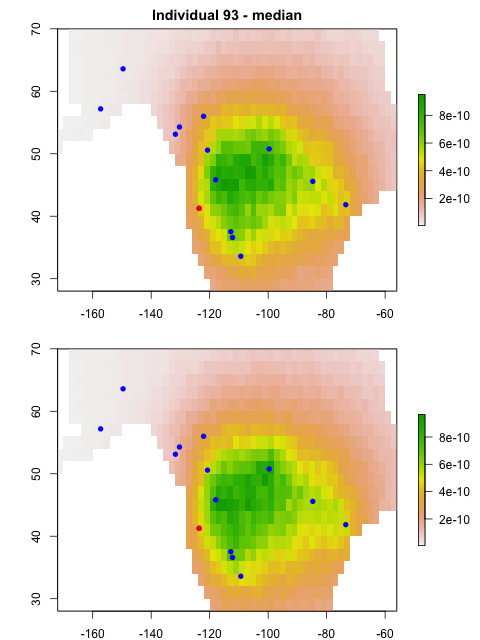
\includegraphics[width=2in]{scat/pics/Ind93-median.png}
\end{frame}

%\begin{frame}
%\begin{center}
%\vspace{-2.75cm}
%\hspace{-2cm}
%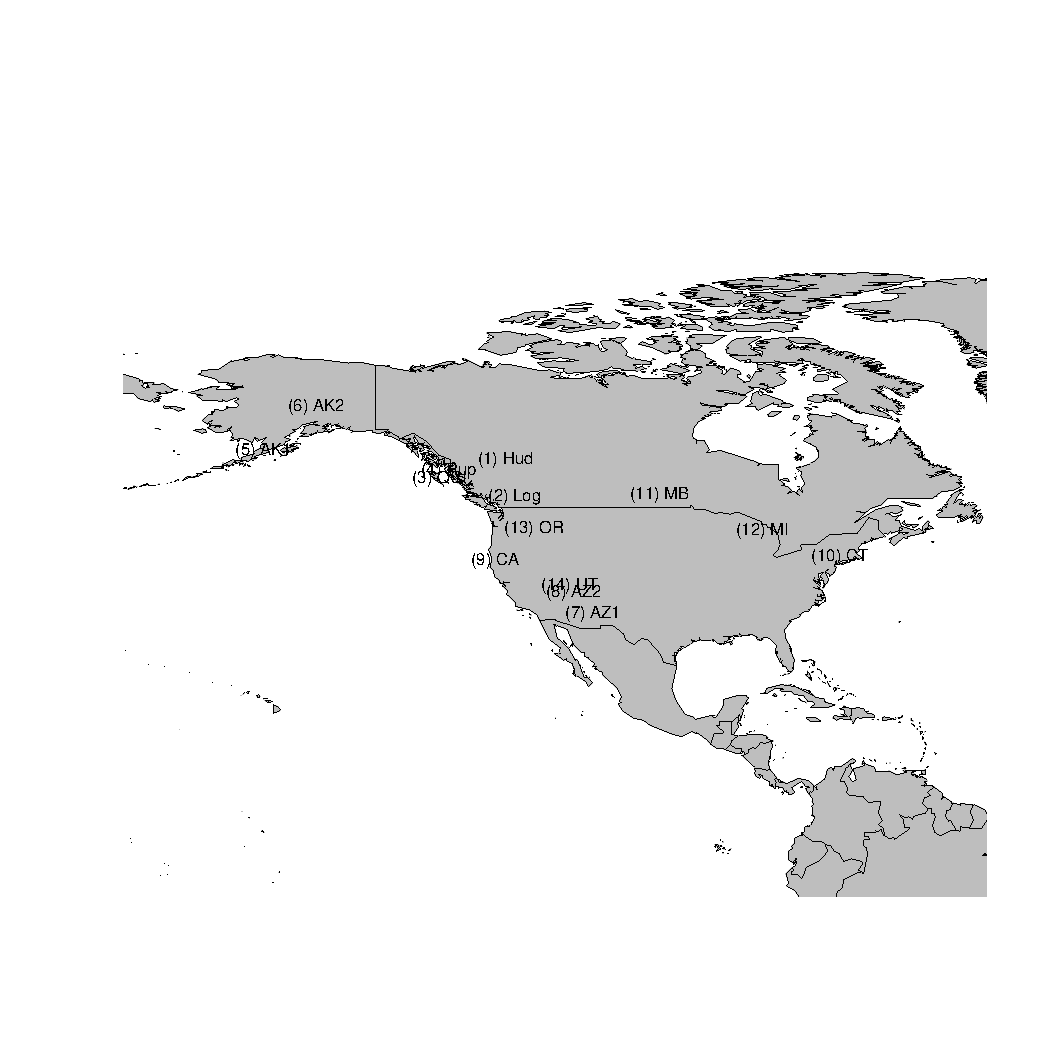
\includegraphics[width=5in]{scat/pics/HETH_locations.pdf}
%\end{center}
%\end{frame}

\begin{frame}
\begin{center}
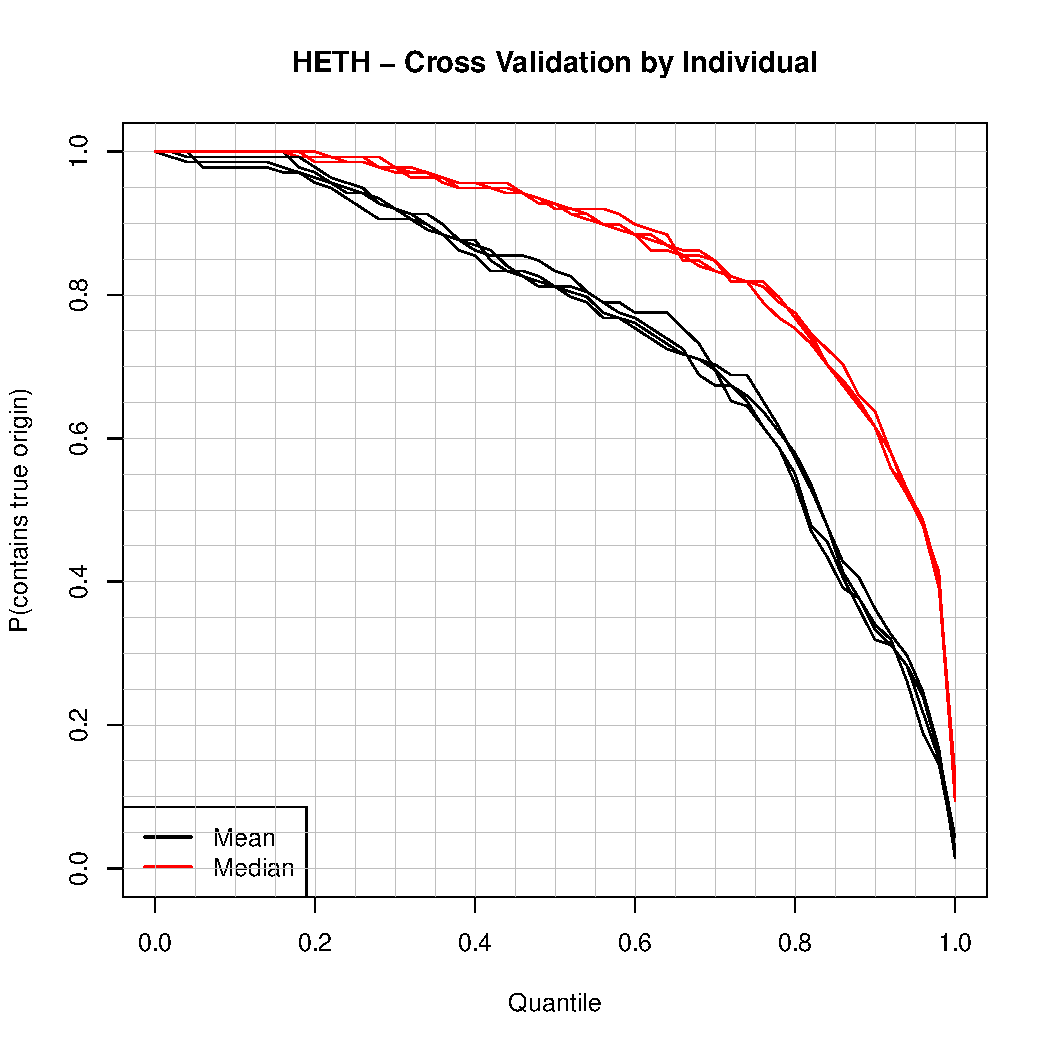
\includegraphics[width=3in]{scat/pics/cover_HETH_Individual.pdf}
\end{center}
\end{frame}

%\begin{frame}
%\begin{center}
%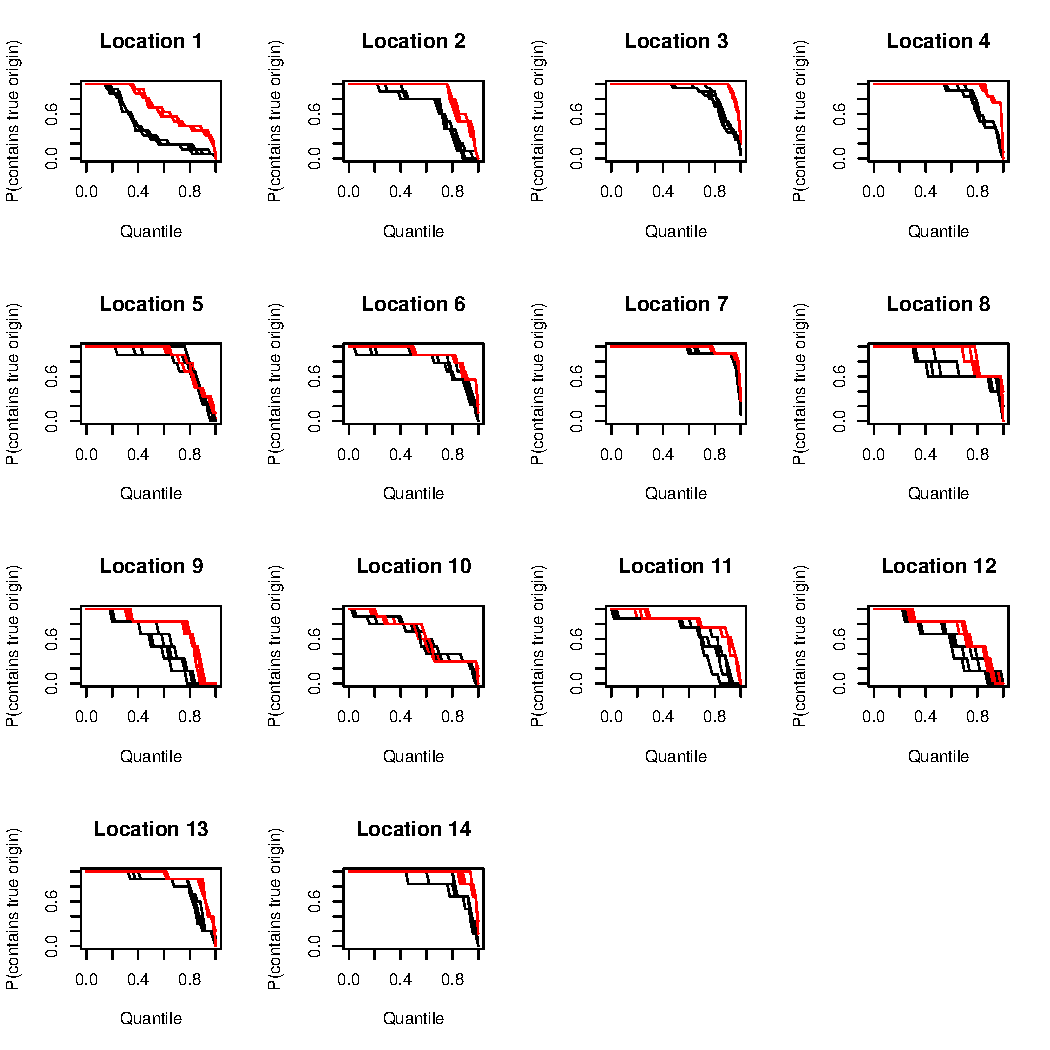
\includegraphics[width=3in]{scat/pics/cover_byloc_HETH_Individual.pdf}
%\end{center}
%\end{frame}


\begin{frame}
\begin{center}
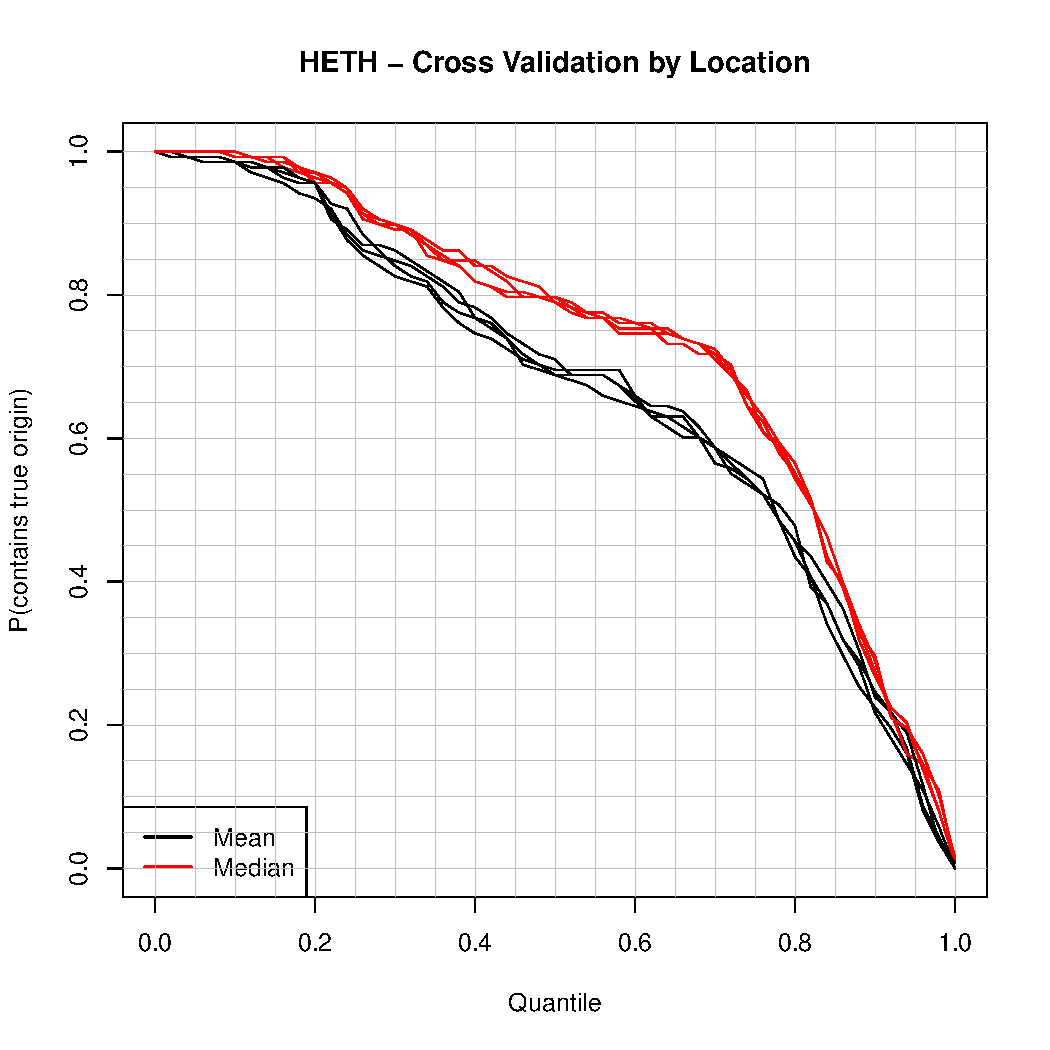
\includegraphics[width=3in]{scat/pics/cover_HETH_Location.pdf}
\end{center}
\end{frame}

%\begin{frame}
%\begin{center}
%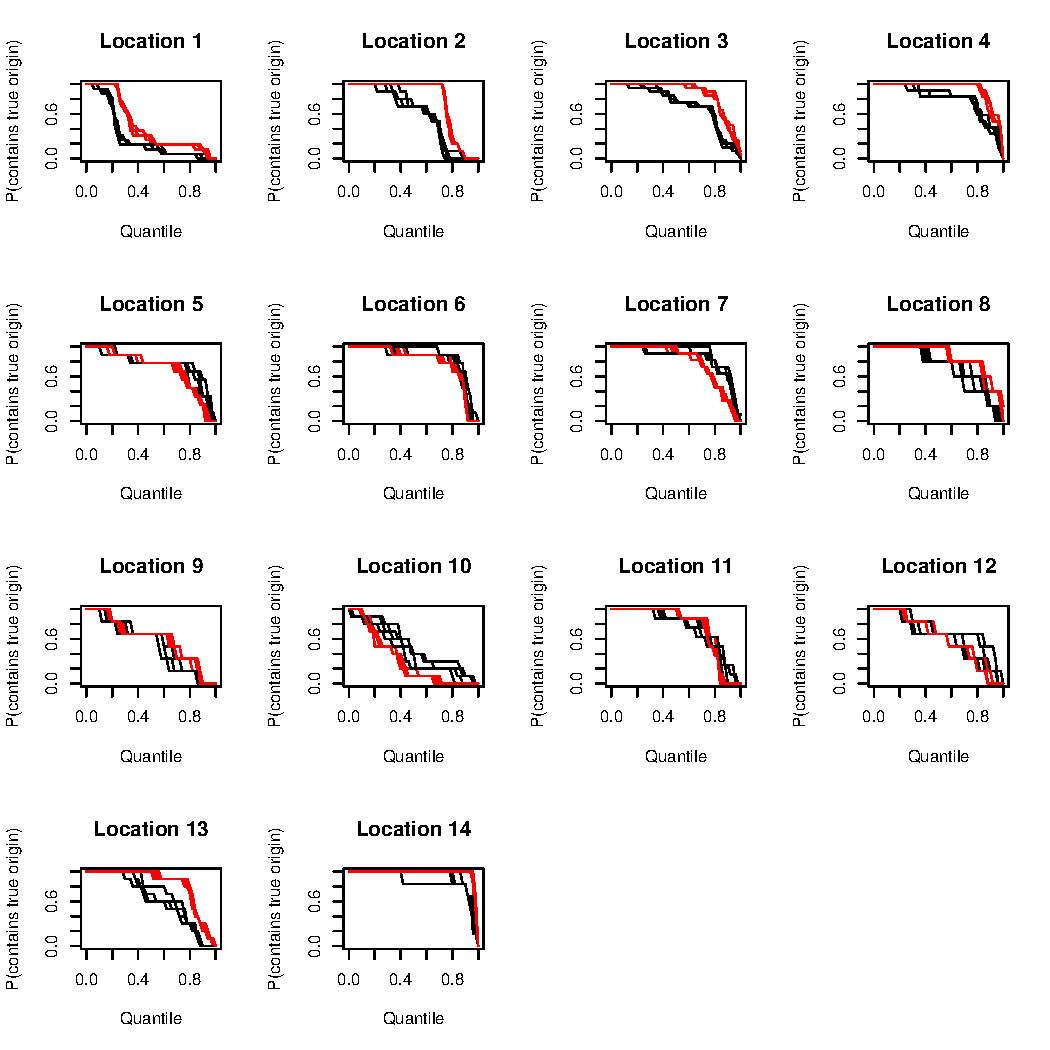
\includegraphics[width=3in]{scat/pics/cover_byloc_HETH_Location.pdf}
%\end{center}
%\end{frame}

%% --------------------------------------------------- 
%% SWTH
%% --------------------------------------------------- 
%
%\section{Swainson's Thrush}
%\subsection{}
%
%\begin{frame}
%\begin{center}
%\vspace{-1.5cm}
%\hspace{-1cm}
%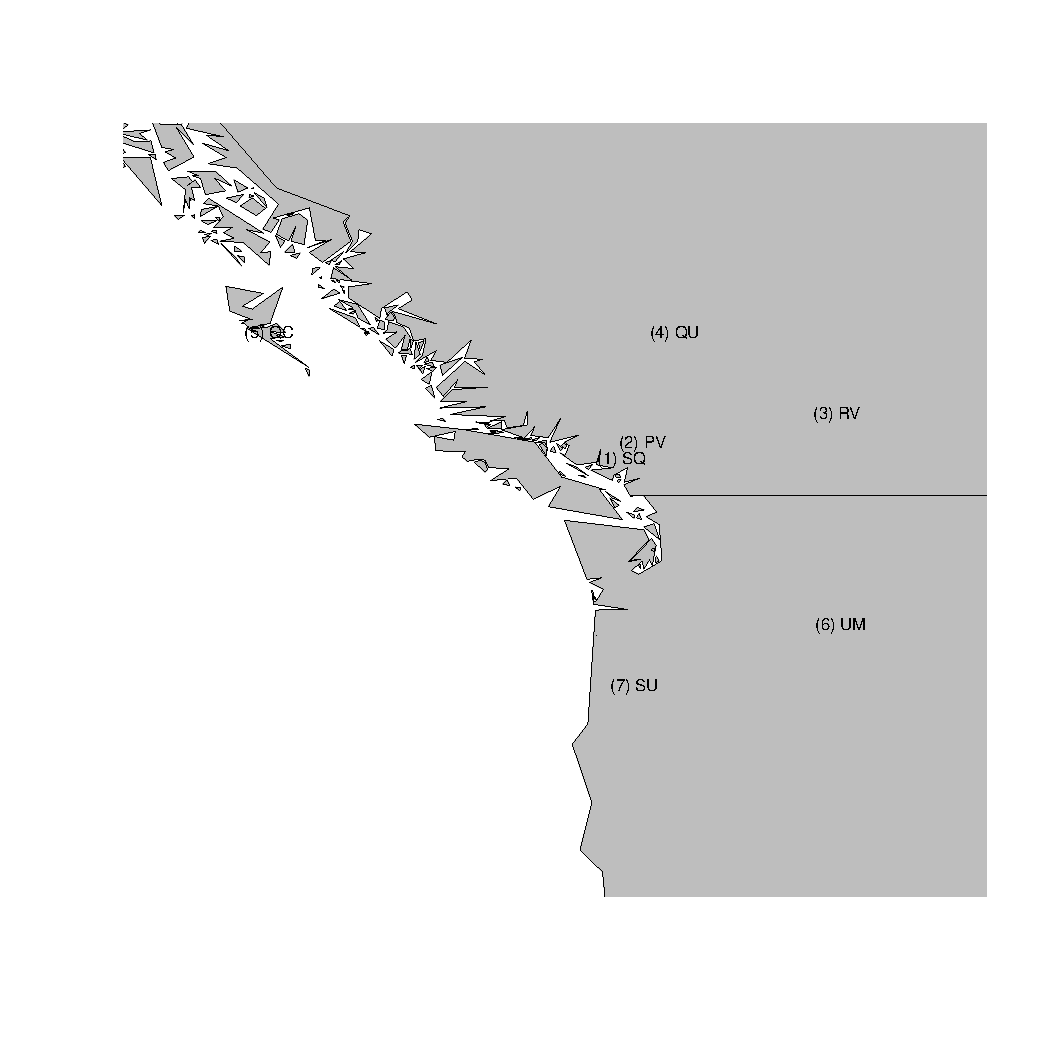
\includegraphics[width=4.5in]{scat/pics/SWTH_locations.pdf}
%\end{center}
%\end{frame}
%
%\begin{frame}
%\begin{center}
%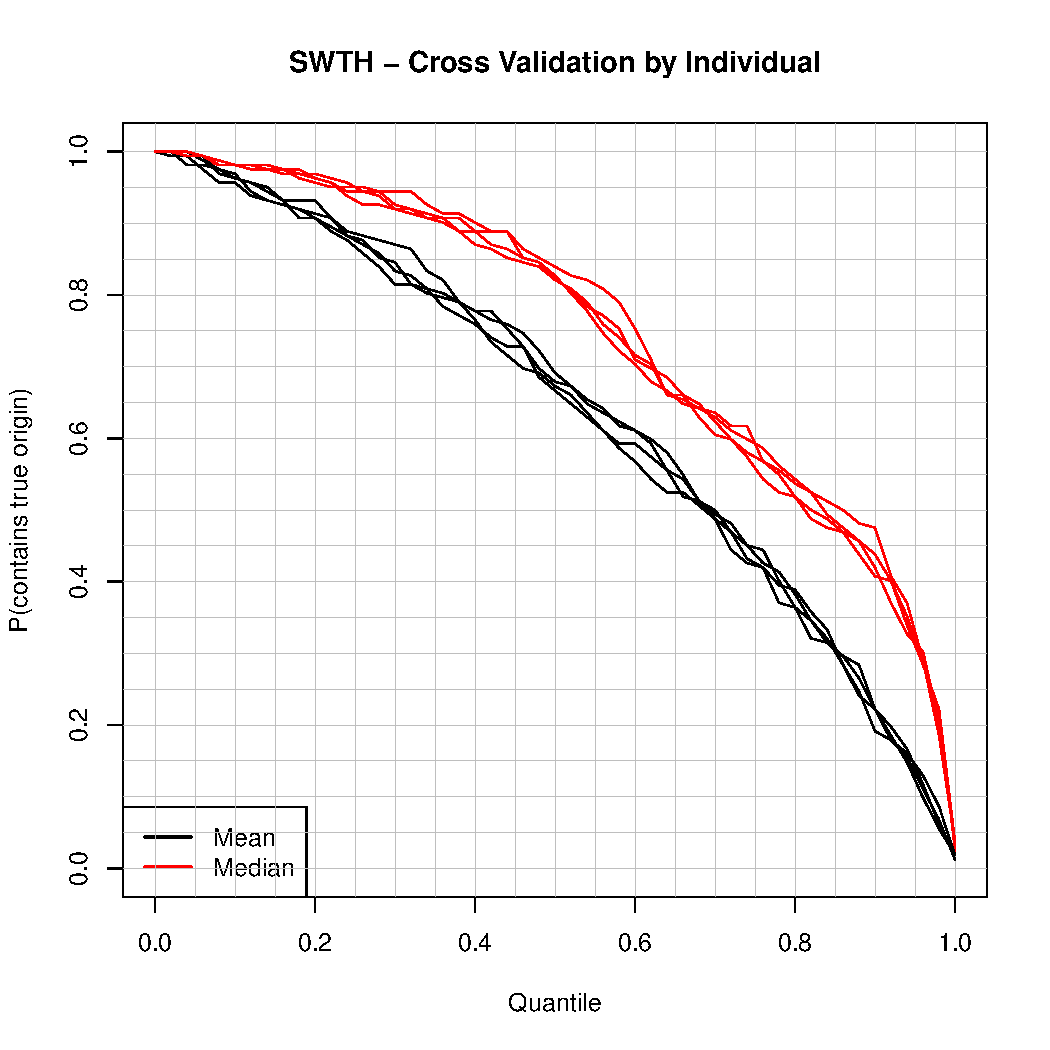
\includegraphics[width=3in]{scat/pics/cover_SWTH_Individual.pdf}
%\end{center}
%\end{frame}
%
%\begin{frame}
%\begin{center}
%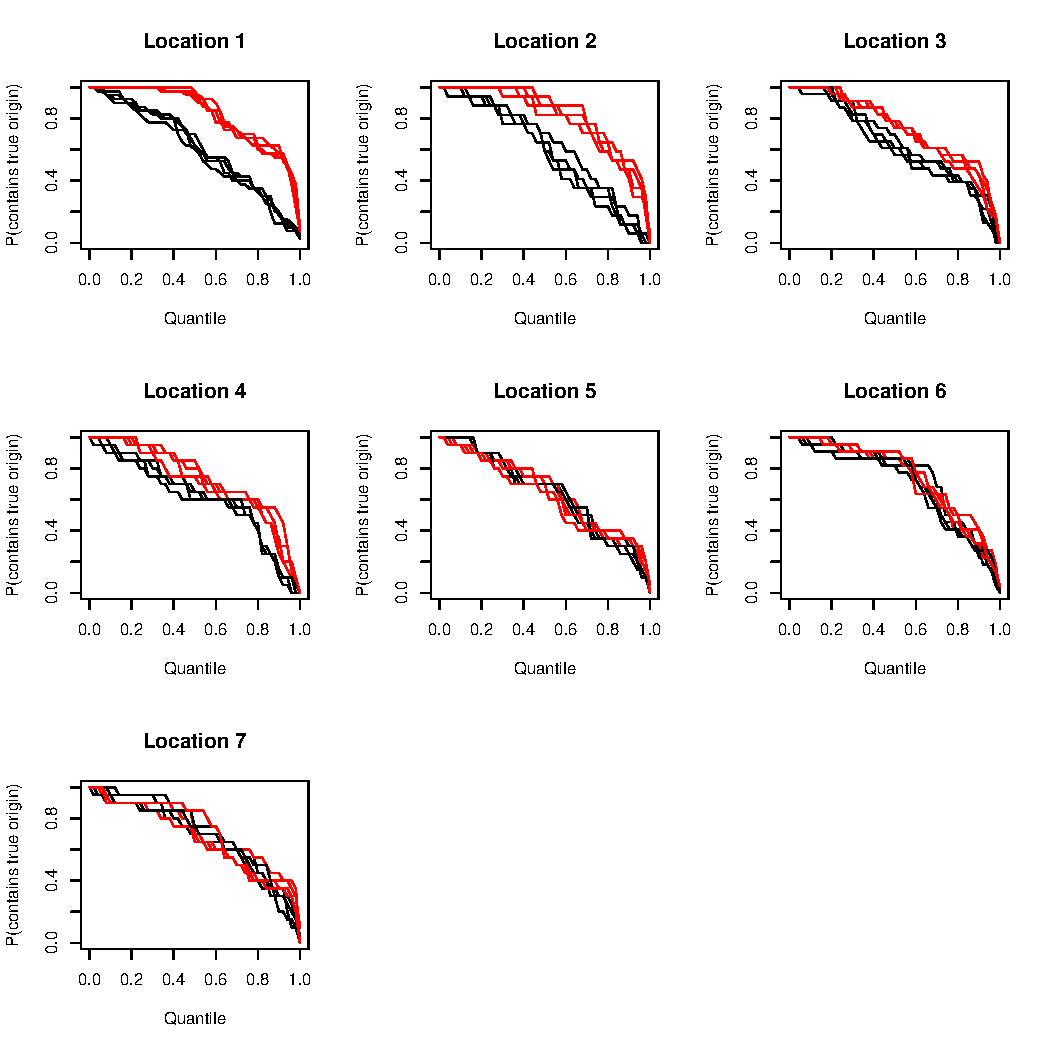
\includegraphics[width=3in]{scat/pics/cover_byloc_SWTH_Individual.pdf}
%\end{center}
%\end{frame}
%
%
%\begin{frame}
%\begin{center}
%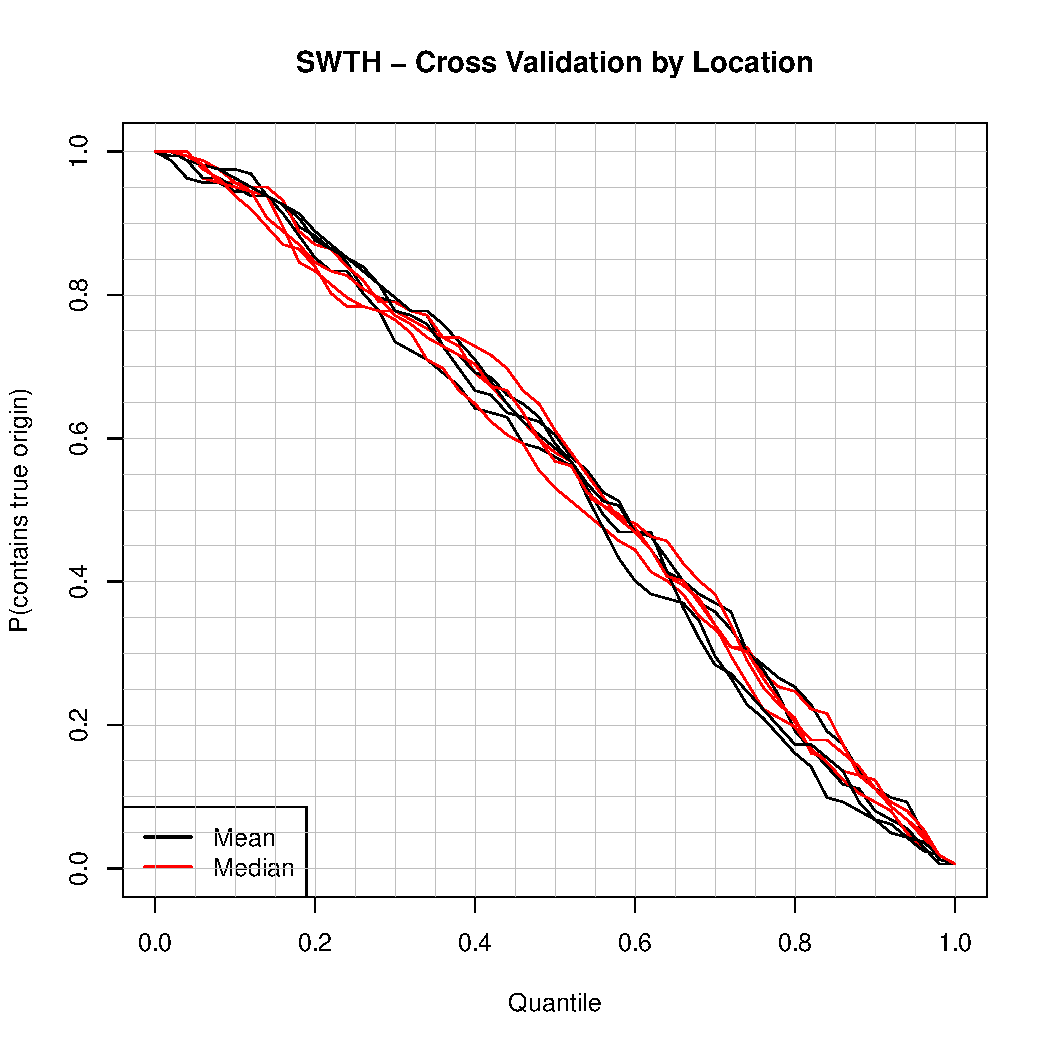
\includegraphics[width=3in]{scat/pics/cover_SWTH_Location.pdf}
%\end{center}
%\end{frame}
%
%\begin{frame}
%\begin{center}
%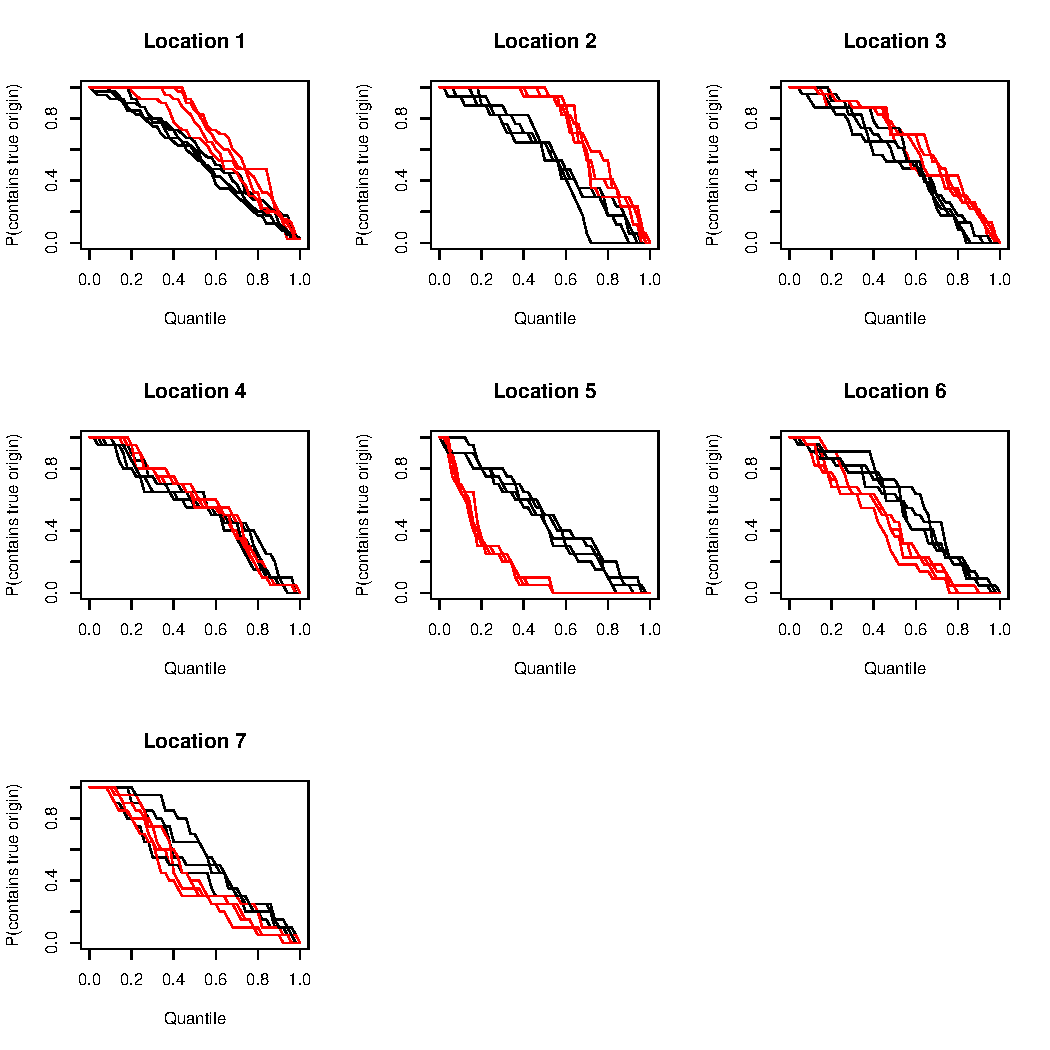
\includegraphics[width=3in]{scat/pics/cover_byloc_SWTH_Location.pdf}
%\end{center}
%\end{frame}
%
%
%% --------------------------------------------------- 
%% WIWA
%% --------------------------------------------------- 
%
%\section{Wilson's Warbler}
%\subsection{}
%
%\begin{frame}
%\begin{center}
%\vspace{-1.5cm}
%\hspace{-1cm}
%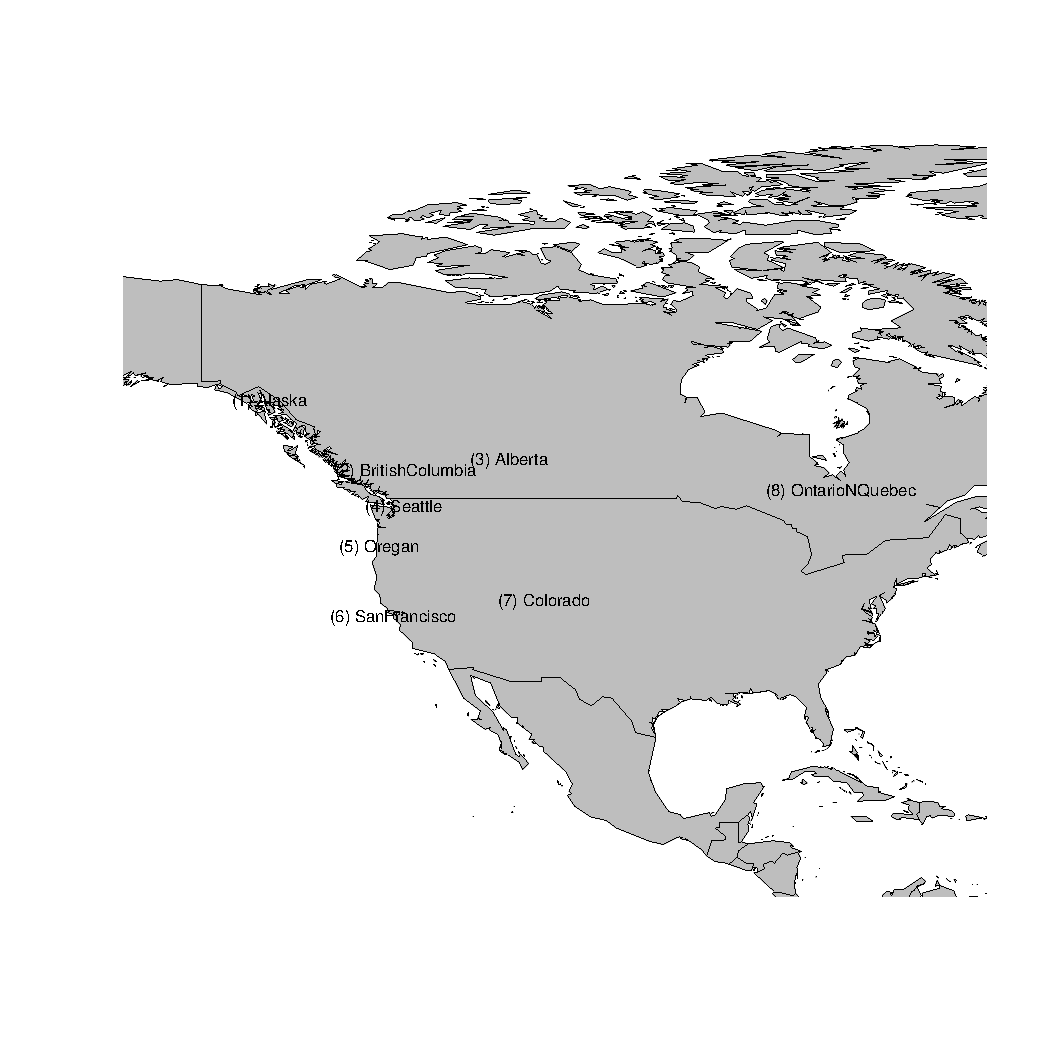
\includegraphics[width=4.5in]{scat/pics/WIWA_locations.pdf}
%\end{center}
%\end{frame}
%
%
%\begin{frame}
%\begin{center}
%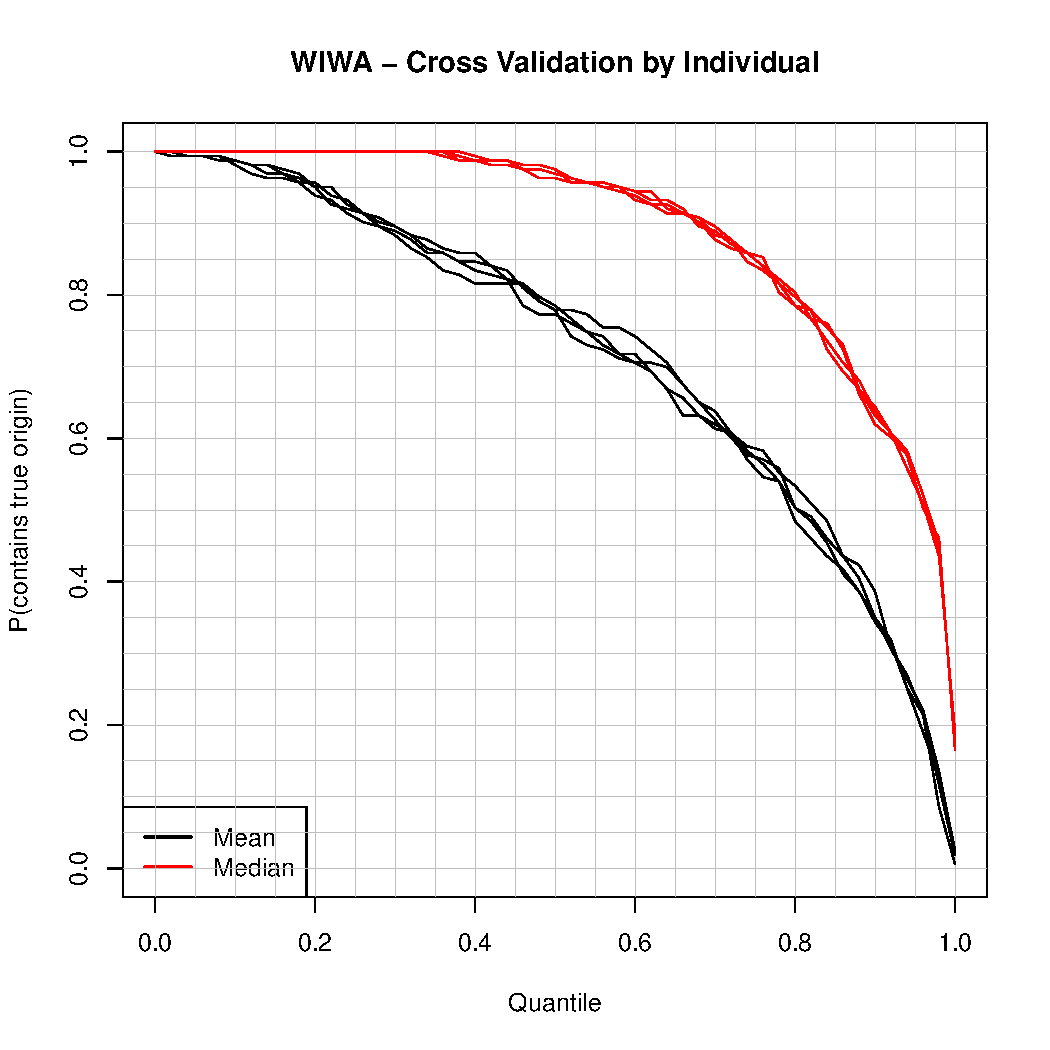
\includegraphics[width=3in]{scat/pics/cover_WIWA_Individual.pdf}
%\end{center}
%\end{frame}
%
%\begin{frame}
%\begin{center}
%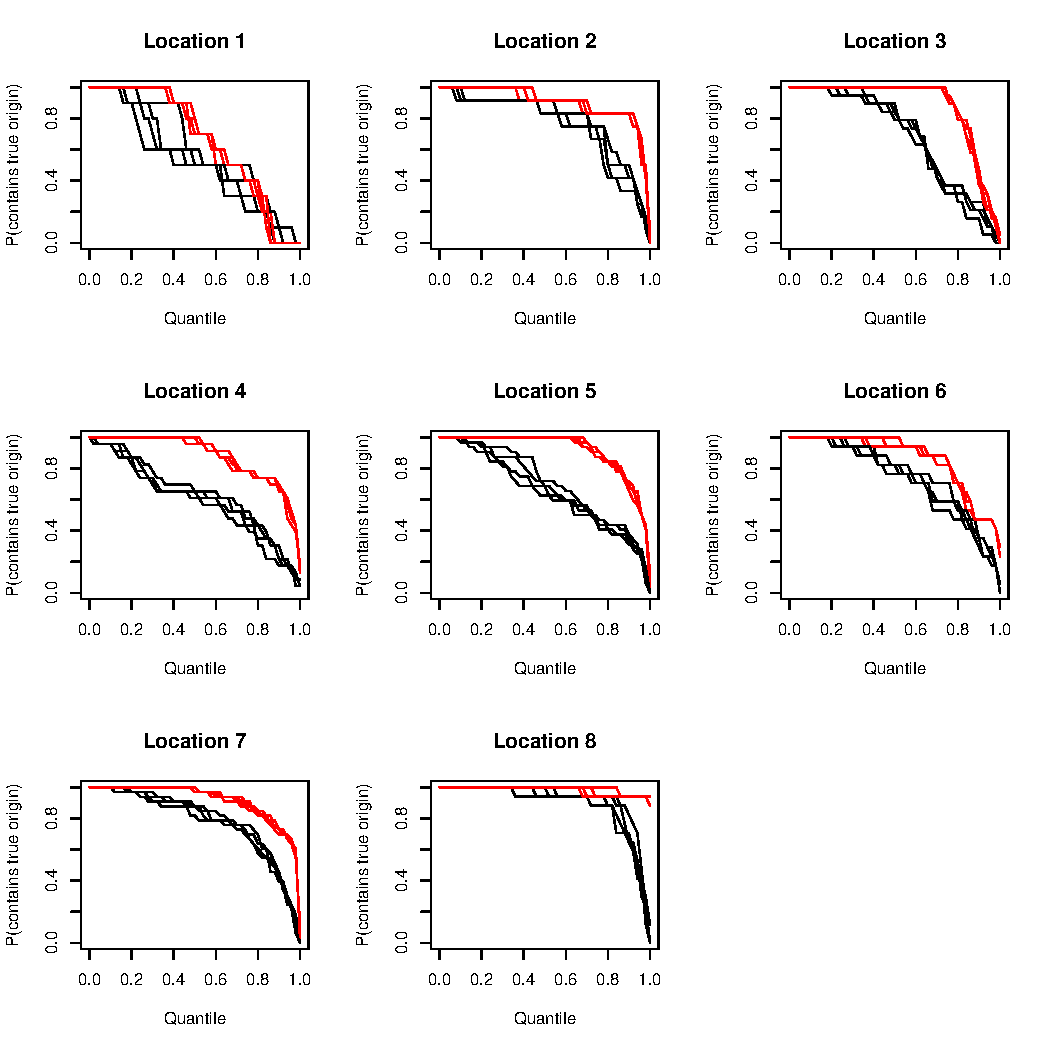
\includegraphics[width=3in]{scat/pics/cover_byloc_WIWA_Individual.pdf}
%\end{center}
%\end{frame}
%
%
%\begin{frame}
%\begin{center}
%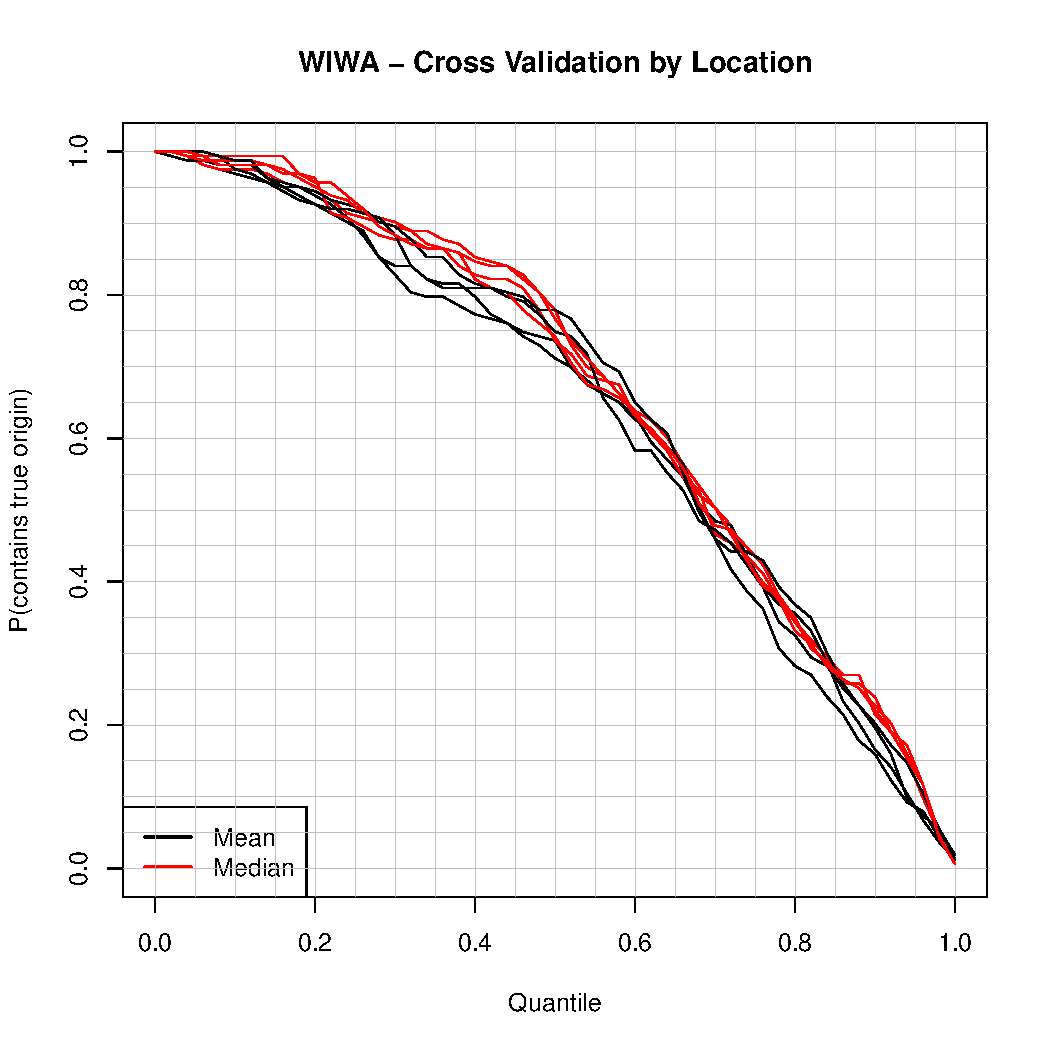
\includegraphics[width=3in]{scat/pics/cover_WIWA_Location.pdf}
%\end{center}
%\end{frame}
%
%\begin{frame}
%\begin{center}
%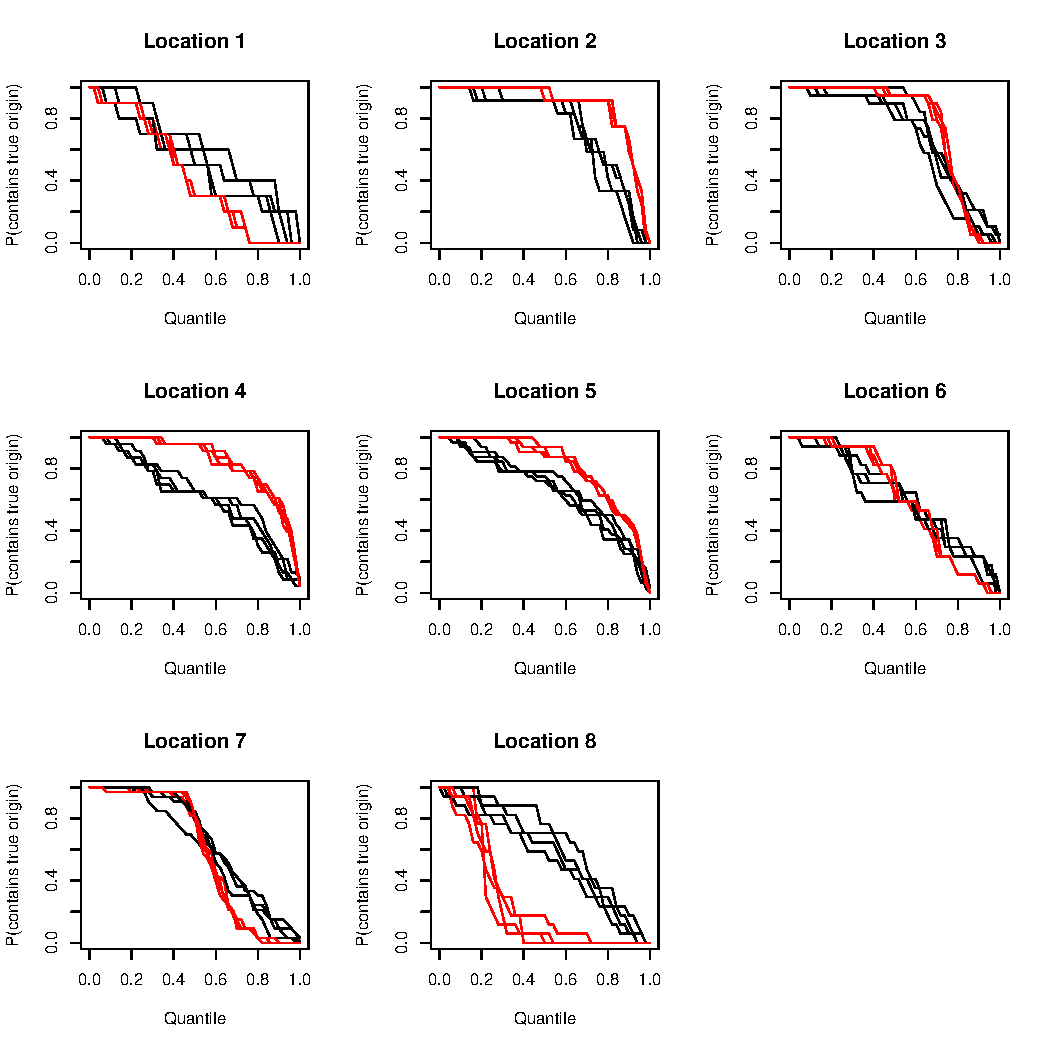
\includegraphics[width=3in]{scat/pics/cover_byloc_WIWA_Location.pdf}
%\end{center}
%\end{frame}


